\medskip

La \textbf{partie C} est indépendante des parties \textbf{A} et \textbf{B}.

\medskip

\textbf{Partie A}

\medskip

On donne ci-dessous, dans un repère orthogonal, les courbes $\mathcal{C}_{1}$ et $\mathcal{C}_{2}$, représentations graphiques de deux fonctions définies et dérivables sur $\R$. L'une des deux fonctions représentées est la fonction dérivée de l'autre. On les notera $g$ et $g’$.

On précise également que :
\begin{itemize}
\item La courbe $\mathcal{C}_{1}$ coupe l'axe des ordonnées au point de coordonnées $(0~;~1)$.
\item La courbe $\mathcal{C}_{2}$ coupe l'axe des ordonnées au point de coordonnées $(0~;~2)$ et l'axe des abscisses aux points de coordonnées $(-2~;~0)$ et $(1~;~0)$.
\end{itemize}

\begin{center}
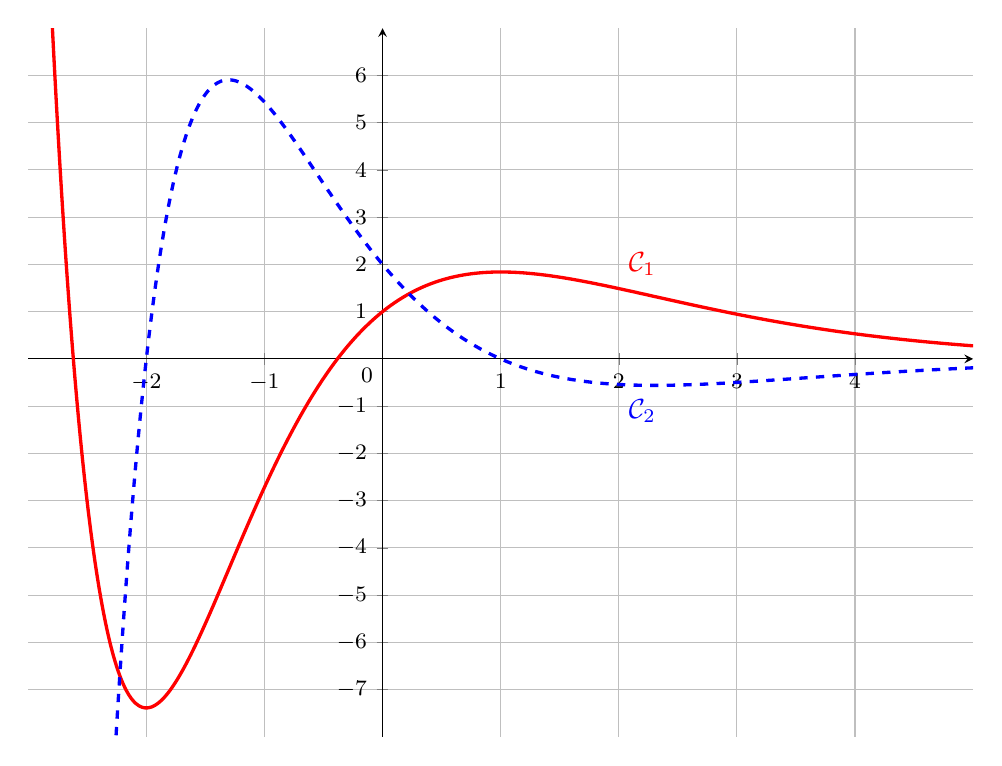
\begin{tikzpicture}
\begin{axis}[/pgf/number format/.cd, use comma,
x={15mm}, y={6mm}, 
xmin=-3, xmax=5, ymin = -8, ymax= 7, 
xtick = {-2,...,4}, ytick={-7,...,6},
tick label style={font=\footnotesize},
minor tick num = 0, grid=major, axis lines =center]
\node[below left] at (axis cs: 0,0) {{\footnotesize 0}};
\addplot [line width=1.2pt, color=red, smooth, samples=300, domain= -3:5]{(x^2+3*x+1)*exp(-x)};
\node[red] at(axis cs: 2.2,2) {$ \mathcal{C}_1 $};
\addplot [line width=1.2pt, color=blue, dashed, smooth, samples=300, domain= -3:5]{(-x^2-x+2)*exp(-x)};
\node[blue] at(axis cs: 2.2,-1.1) {$ \mathcal{C}_2 $};
\end{axis}
\end{tikzpicture}
















\end{center}

\begin{enumerate}
	\item En justifiant, associer à chacune des fonctions $g$ et $g'$ sa représentation graphique.
	\item Justifier que l'équation réduite de la tangente à la
courbe représentative de la fonction $g$ au point d'abscisse 0 est $y=2x + 1$.
\end{enumerate}

\medskip

\textbf{Partie B}

\medskip

On considère $(E)$ l'équation différentielle 

\[y+y'=(2x + 3) \e^{-x},\]
où $y$ est une fonction de la variable réelle $x$.

\medskip

\begin{enumerate}
\item Montrer que la fonction $f_{0}$ définie pour tout nombre réel $x$ par $f_{0}(x)=\left(x^{2}+3 x\right) \e^{-x}$ est une solution particulière de l'équation différentielle $(E)$.
\item Résoudre l'équation différentielle $\left(E_{0}\right): y+ y'= 0$.
\item Déterminer les solutions de l'équation différentielle $(E)$.
\item On admet que la fonction $g$ décrite dans la \textbf{partie A} est une solution de l'équation différentielle $(E)$.

Déterminer alors l'expression de la fonction $g$.
\item Déterminer les solutions de l'équation différentielle $(E)$ dont la courbe admet exactement deux points d'inflexion.
\end{enumerate}

\medskip

\textbf{Partie C}

\medskip

On considère la fonction $f$ définie pour tout nombre réel $x$ par :

\[f(x)=\left(x^{2}+3 x+2\right) \e^{-x}\]

\begin{enumerate}
\item Démontrer que la limite de la fonction $f$ en $+\infty$ est égale à 0.

On admet par ailleurs que la limite de la fonction $f$ en $-\infty$ est égale à $+\infty$.

\item On admet que la fonction $f$ est dérivable sur $\R$. On note $f’$ la fonction dérivée de $f$ sur $\R$.
	\begin{enumerate}
		\item Vérifier que, pour tout nombre réel $x$, $f’(x)=\left(-x^{2}-x+1\right) \e^{-x}$.
		\item Déterminer le signe de la fonction dérivée $f’$ sur $\R$ puis en déduire les variations de la fonction $f$ sur $\R$.
	\end{enumerate}
\item Expliquer pourquoi la fonction $f$ est positive sur l'intervalle $[0;+\infty[$.
\item On notera $\mathcal{C}_{f}$ la courbe représentative de la fonction $f$ dans un repère orthogonal \Oij. On admet que la fonction $F$ définie pour tout nombre réel $x$ par $F(x)=\left(-x^{2}-5 x-7\right) \e^{-x}$ est une primitive de la fonction $f$.

Soit $\alpha$ un nombre réel positif.

Déterminer l'aire $\mathcal{A}(\alpha)$, exprimée en unité d'aire, du domaine du plan délimité par l'axe des abscisses, la courbe $\mathcal{C}_{f}$ et les droites d'équation $x=0$ et $x=\alpha$.
\end{enumerate}
